%%%%%%%%%%%%%%%%%%%%%%%%%%%%%%%%%%%%%%%%%%%%%%%%%%%%%%%%%%%%%

\mainmatter
\setcounter{page}{1}

\lectureseries[\course]{\course}

\auth[\lecAuth]{Lecturer: \lecAuth\\ Scribe: \scribe}
\date{November 24, 2009}

\setaddress

% the following hack starts the lecture numbering at 17
\setcounter{lecture}{16}
\setcounter{chapter}{16}

\lecture{Frequency Domain Analysis}

\section{Approximate Modeling Review}
An approximate model is generated when $\mathcal{S}\notin\mathcal{M}$. This gives a best available approximation of the parameters as
$$\theta^\ast = \argmin_\theta \bar{V}(\theta) = \argmin_\theta\bar{E}\{\est\} \text{ w.p. } 1$$
We can only compute $\tast$ by hand for small models. However, Parceval's theorem shows that
\begin{align*}
\tast &= \argmin_\theta \frac{1}{2\pi}\int_{-\pi}^\pi \Phi_\eps(\w,\theta)d\w \\
\Phi_\eps(\w,\theta) &= \frac{|G_0(e^{j\w})-G_\theta(e^{j\w})|^2\Phi_u(\w) + |H_0(e^{j\w})-H_\theta(e^{j\w})|^2\lambda}{|H_\theta(e^{j\w}|^2}
\end{align*}
For open loop systems $\Phi_{ue}(\w) = 0$. This gives a qualitative expression for what $\tast$ represents using
\begin{itemize}
\item Input spectrum.
\item Model structure.
\item $L(q)$ to influence model fit.
\end{itemize}
Notice that there is a trade-off between modeling the deterministic portion (system dynamics in $G_0$ and $G_\theta$) and noise ($H_0$ and $H_\theta$). In this expression the denominator $|H_\theta(e^{j\w})|^2$ supplies an implicit weighting term. Also, this is a biased model because $G_\theta\not\to G_0$.

\section{Frequency Domain Data}
If we know the bias forumla from the frequency domain then why not directly fit a model in the frequency domain? We start with $\hat{G}(e^{j\w}) \triangleq$ frequency domain data of $G_0(e^{j\w})$. How do we obtain frequency domain data for $\hat{G}(e^{j\w})$ using the signals $\{u(t),y(t)\}$? Use either the empirical transfer function estimate (ETFE) or spectral analysis (SPA) as discussed in Lecture \ref{lec:7}.
\begin{itemize}
\item ETFE:
$$\hat{\hat{G}}^N(e^{j\w}) = \frac{Y_N(\w)}{U_N(\w)}$$
\item Spectral analysis:
$$\hat{G}^N(e^{j\w}) = \frac{\int Y_N(\xi)W(\w-\xi)d\xi}{\int U_N(\xi)W(\w-\xi)d\xi}$$
\end{itemize}
Properties of the ETFE include
\begin{itemize}
\item $$\lim_{N\to\infty}E\left\lbrace \hat{\hat{G}}(e^{j\w})\right\rbrace = G_0(e^{j\w})$$
\item $$\lim_{N\to\infty}E\left\lbrace (\hat{\hat{G}}^N-G_0)^2\right\rbrace = \left|\hat{\hat{G}}(e^{j\w})\right|^2$$
\end{itemize}
Properties of SPA include
\begin{itemize}
\item $$\lim_{N\to\infty}E\left\lbrace (\hat{G}^N-G_0)^2\right\rbrace = 0$$
\item There is no bias in the estimate, $\var\to0$.
\end{itemize}
The procedure involves estimating the covariance such that
\begin{align*}
\hat{R}_{yu}^N(\tau) &= \frac{1}{N}\sumt y(t)u(t-\tau) \\
\bar{R}_{yu}^N(\tau) &= \hat{R}_{yu}^N(\tau)\cdot W(\tau) \\
\hat{\Phi}_{yu}(\w) &= \mathcal{F}\left\lbrace \bar{R}_{yu}^N(\tau)\right\rbrace = \int\bar{\Phi}_{yu}(\xi) W(\w-\xi)d\w
\end{align*}
where $W(\w) = \mathcal{F}\{W(\tau)\}$. Then we have that
$$\hat{G}_{\text{spa}}\ejw = \frac{\hat{\Phi}_{yu}(\w)}{\hat{\Phi}_u(\w)}$$
Note that this is \textit{not} a model!

\section{Frequency Domain Identification}
Starting with $\hat{G}\ejw$ we get a frequency domain representation of the data of $G_0\ejw$. From here, how do we get a model $P(e^{j\w},\theta)$? A more formal way of stating this is that
$$\Omega = \left\lbrace \w ~|~ \w=\w_k, \w_k=\frac{k\cdot 2\pi}{T} \right\rbrace$$
is a frequency grid where $T=N\cdot\Delta T$. This means that the longer measurements are recorded the finer the resolution of the frequency grid.

Now, define the additive error as
$$E_a(\w,\theta) \triangleq |\hat{G}\ejw-P(e^{j\w},\theta)|, \qquad \w\in\Omega$$
We could also use element-wise multiplication to get weighted errors in the multivariable case. The element-wise multiplication is known as a Schur product and the \textsc{Matlab} notation is `\texttt{.*}'. This gives
$$E_s(\w,\theta) = (\hat{G}\ejw-P(e^{j\w},\theta)).*S(\w)$$
Either method gives $E(\w)$. This lets us formulate a least squares problem in the frequency domain such that
\begin{align}
\label{eq:17fls}
\hat{\theta} = \argmin_\theta\sum_{k=1}^N\text{tr}\left\lbrace E(\w_k,\theta)E^\ast(\w_k,\theta)\right\rbrace
\end{align}
Note that, for $E_a$ we have $\hat{G},P\in\mathbb{C}$.

\subsection{Solvability of Least Squares}
The solvability of (\ref{eq:17fls}) depends on $P(e^{j\w},\theta)$ or the parameterization of the model. A simple case can be illustrated by using an FIR model to get
\begin{align*}
P(q,\theta) &= \sumk b_0q^{-k} \\
P(e^{j\w},\theta) &\stackrel{\text{z-transform}}{=} \sumk b_\theta z^{-k} \stackrel{\mathcal{L}\{\}}{=} \sumk b_0e^{-j\w k} \\
&= b_0 + b_1e^{-j\w} + b_2e^{-j\w 2} + \ldots + b_ne^{-j\w n} \\
&= [1 ~ e^{-j\w} ~ e^{-j\w 2} ~ \cdots ~ e^{-j\w n}] \cdot [b_0 ~ b_1 ~ b_2 ~ \ldots ~ b_n]^T \\
&= \vp(\w)^T\theta \\
\Rightarrow P(e^{j\w},\theta) &= \vp^T(\w)\theta \\
\Rightarrow E(\w,\theta) &= \hat{G}\ejw-\vp^T(\w)\theta
\end{align*}
with $\hat{G}$ from ETFE or SPA. This leads to
$$\min_\theta|E(\theta)|_2^2$$
and can be solved using least squares, projection or $\tfrac{\partial}{\partial\theta}(\cdot)=0$ to get
$$\sumk\vp(\w_k)E(\w_k,\theta) = \sumk\vp(\w_k)\hat{G}(e^{j\w_k}) - \sumk\vp(\w_k)\vp^T(\w_k)\theta$$
The inner product of the regressor and the error is then eliminated yielding
$$\thn = \left[\fN\sumk\vp(\w_k)\vp^T(\w_k)\right]^{-1}\left[\fN\sumk\vp(\w_k)\hat{G}(e^{j\w_k})\right]$$
This is a least squares solution for an FIR model.

We can see that $\vp(\w_k)\in\mathbb{C}$, $\hat{G}(e^{j\w_k})\in\mathbb{C}$ so $\thn\in\mathbb{C}$. To avoid $\thn\in\mathbb{C}$ we can split the error into real and imaginary components such that
$$E(\w,\theta) = \left[\text{Re}\{E(\w,\theta)\} \qquad \text{Im}\{E(\w,\theta)\}\right]$$
and do that for both $\vp(\w)$ and $\hat{G}\ejw$ as well.

The conclusion is that the same type of least squares solution is possible but the complex numbers need to be split up into real and imaginary parts to ensure that $\thn\in\mathbb{R}$. However, a least squares solution using frequency domain data is only possible if $G(\w,\theta)$ is an FIR model.

\section{Comparison with Time Domain}
In the time domain both FIR and ARX models yielded a least squares solution. To compare the time domain and the frequency domain representations we can look at the system
$$\mathcal{S}: y(t) = G_0(q)u(t) + v(t)$$

The error of a time domain model for this system is
\begin{align*}
y(t) &= \gt u(t)+\hth\ett \\
y(t) &= \frac{B_\theta(q)}{A_\theta(q)}u(t) + \frac{1}{A_\theta(q)}\ett \\
\ett &= B_\theta(q)u(t) - A_\theta(q)y(t)
\end{align*}
while the frequency domain gives
\begin{align*}
\hat{G}\ejw &= G_0\ejw + N\ejw \\
\Phi_{yu}(\w) &= G_0\ejw\Phi_u(\w) + \Phi_{uv}(\w) \\
\Rightarrow \frac{\hat{\Phi}_{yu}(\w)}{\hat{\Phi}_u(\w)} &= G_0\ejw + \frac{\hat{\Phi}_{uv}(\w)}{\hat{\Phi}_u(\w)}
\end{align*}
Notice that there is no noise model in the frequency domain!
$$E(\w,\theta) = \hat{G}\ejw - \tilde{G}\ejw$$
which is similar in form to an output error (OE) model in the time domain.

The conclusion is that in frequency domain curve-fitting only OE models can be used which means that it is only a least squares problem if for
$$G(e^{j\w},\theta) = \frac{B(e^{j\w},\theta)}{F(e^{j\w},\theta)}$$
we have $F(e^{j\w},\theta) = 1$ giving the result that $G(e^{j\w},\theta)$ has to be an FIR model.

Fitting in the frequency domain must always be performed using an OE model and thus always requires non-linear optimization. However, it can provide a nice visual confirmation of whether the model is a good fit as opposed to least squares in the time domain which does not give any visual confirmation.

\section{Iterative Linear Techniques}
The algorithm we will get at the end of this section is known as the Sanathanan and Koerner iteration. We want to minimize the output error using
$$E(\w,\theta) = \hat{G}\ejw - \frac{B(e^{j\w},\theta)}{F(e^{j\w},\theta)}$$
using non-linear optimization. First, we get the equation error as
\begin{align*}
\tilde{E}(\w,\theta) &= F(e^{j\w},\theta)E(\w,\theta) \\
&= F(e^{j\w},\theta)\cdot\tilde{G}\ejw - B(e^{j\w},\theta)
\end{align*}
Using the property that $F(e^{j\w},\theta)$ is monic we get
\begin{align*}
F(e^{j\w},\theta) &= 1 + f_1e^{-j\w} + f_2e^{-2j\w} + \ldots \\
\tilde{E}(\w,\theta) &= \hat{G}\ejw - \vp^T(\w)\theta \\
\vp^T(\w) &= [1 ~ e^{-j\w} ~ e^{-2j\w} ~ \cdots ~ -e^{-j\w}\hat{G}\ejw ~ -e^{-2j\w}\hat{G}\ejw ~ \cdots] \\
\theta^T &= [b_0 ~ b_1 ~ b_2 ~ \cdots ~ b_{n_b} ~ f_1 ~ f_2 ~ \cdots ~ f_{n_f}]
\end{align*}
If
\begin{align*}
\hat{\theta} &= \argmin_\theta \fN\sumk\tilde{E}(\w_k,\theta)\tilde{E}^T(\w_k,\theta) \\
&= \left[\fN\sumk\vp(\w)\vp^T(\w)\right]^{-1}\left[\fN\sumk\vp(\w)\hat{G}\ejw\right]
\end{align*}
with
\begin{align*}
\vp(\w) &= [\text{Re}\{\vp(\w)\} \qquad \text{Im}\{\vp(\w)\}] \\
\hat{G}\ejw &= [\text{Re}\{\hat{G}\ejw\} \qquad \text{Im}\{\hat{G}\ejw\}]
\end{align*}
However,
\begin{align*}
\hat{\theta} &= \argmin_\theta \left|F(e^{j\w},\theta)\hat{G}\ejw - B(e^{j\w},\theta)\right|_2 \\
&= \argmin_\theta \left|F(e^{j\w},\theta)\left[\underbrace{\hat{G}\ejw - \frac{B(e^{j\w},\theta)}{F(e^{j\w},\theta)}}_{\text{OE}}\right]\right|_2
\end{align*}
Note that $F(e^{j\w},\theta)$ is an implicit weighting function.

This is similar to ARX where the implicit weighting function brings out the high-frequency response. In Figure \ref{fig:17poles} we see that the response increases at the poles of the system.

The conclusion is that fitting frequency data using least squares (minimizing the equation error) leads to a fit with an implicit high-frequency emphasis.

\begin{figure}[ht!]
	\centering
	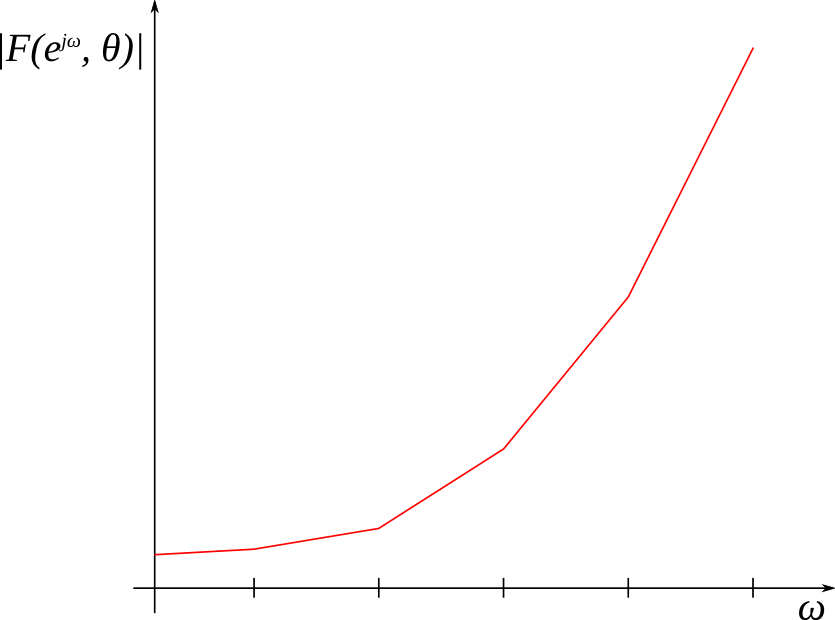
\includegraphics[width=.4\textwidth]{images/17poles}
	\caption{Implicit high-frequency weighting.}
	\label{fig:17poles}
\end{figure}

\begin{example}
Using a high order system with a response and estimate as shown in Figure \ref{fig:17model} we get a noisy estimate because
\begin{itemize}
\item There is usually noise at high frequencies.
\item $G_0\ejw\to0$ as $\w\to\infty$.
\end{itemize}
Since we are looking at a log scale small errors will look bigger as well. When fitting a least squares model using the equation error minimization in the frequency domain using a $2$nd order model with $\mathcal{S}\notin\mathcal{M}$
\begin{itemize}
\item The model will try to emphasize a better fit at high frequencies so it is likely we will just model high-frequency noise. If we are lucky we will model the first, largest resonant mode.
\item Typically we will get bad results due to the implicit high-frequency weighting.
\end{itemize}
Ideally, in the frequency domain we would create a weighting function of $\tfrac{1}{F}$ and get
\begin{align*}
\hat{\theta}_{LS} &= \argmin_\theta\tilde{E}(\w) \\
&= \argmin_\theta\tilde{E}_w(\w)
\end{align*}
where
$$\tilde{E}_w(\w) = \frac{1}{F(e^{j\w},\theta)}\tilde{E}(\w,\theta)$$
$\lozenge$
\end{example}

\begin{figure}[ht!]
	\centering
	\includegraphics[width=.4\textwidth]{images/17model}
	\caption{High order system and model response.}
	\label{fig:17model}
\end{figure}

\subsection{Sanathanan and Koerner Iteration}
The Sanathanan and Koerner iteration is given by
\begin{align*}
\boxed{\tilde{E}_w(\w,\theta_i) = \frac{1}{F(e^{j\w},\theta_{i-1})}\tilde{E}(\w,\theta_{i-1})}
\end{align*}
If this converges then we have the filter we want and we will have minimized the OE model error for $\thn$. Note that there is no guarantee of convergence. The normal procedure is to try a few iterations and look at the results. This algorithm is used to eliminate the high-frequency implicit weighting.

\subsection{Relation with Time and Frequency Domain Identification}
In the frequency domain we have
\begin{align*}
\min_\theta\left|\hat{G}(e^{j\w_k}) - \frac{B(e^{j\w_k},\theta)}{F(e^{j\w_k},\theta)}\right|_2, \qquad \w_k\in\Omega
\end{align*}
and in the time domain we have
\begin{align*}
\min_\theta\int\frac{|G_0\ejw-G_\theta\ejw|^2\Phi_u(\w) + |H_0\ejw-H_\theta\ejw|^2}{|H_\theta\ejw|^2}d\w
\end{align*}
When do these two interpretations approach each other?
\begin{itemize}
\item As $N\to\infty$, or when the data sets are large enough that Parceval's theorem holds and $\hat{G}\ejw\to G_0$.
\item Use an OE model in the time domain.
\item $\{u(t)\}$ is white noise so that $\Phi_u(\w)$ is constant.
\end{itemize}
%%%%%%%%%%%%%%%%%%%%%%%%%%%%%%%%%%%%%%%%%%%%%%%%%%%%%%%%%%%%%